%!TEX root = *.tex
%%%%%%%%%%%%%%%%%%
% カウンタのリセット
\setcounter{figure}{0}
% 問題文
図1のように,両端が固定された長さの$l$の弦が水平に張られており,弦の下には水を入れた管が鉛直に立てられている.
この弦の中央をはじき,弦の基本振動により音波を生じさせる.
その状態で,図2のように,水面を管口Aから徐々に下げていくと,Bの位置ではじめて管の中の気柱が音波と共鳴し,Cの位置で2度目の共鳴をした.
Aの位置からBの位置までの距離を$d_1$,Aの位置からCの位置までの距離を$d_2$,弦を伝わる波の速さを$V$とする.
開口端補正を一定として,以下の問いに答えよ.

\begin{enumerate}[(1)]
  \setlength{\leftskip}{-1.5zw}
  \setlength{\itemindent}{1zw}\setlength{\labelsep}{0.5zw}
  \setlength{\labelwidth}{1zw}\setlength{\leftmargin}{1zw}
  \setlength{\itemsep}{0.5\baselineskip}
  \item 弦を伝わる波の波長を求めよ.
  \item 音波の伝わる速さと開口端補正を求めよ.
\end{enumerate}

さらに水面を下げていくと,3度目の共鳴が起こった.

\begin{enumerate}[(1)]
  \setlength{\leftskip}{-1.5zw}
  \setlength{\itemindent}{1zw}\setlength{\labelsep}{0.5zw}
  \setlength{\labelwidth}{1zw}\setlength{\leftmargin}{1zw}
  \setlength{\itemsep}{0.5\baselineskip}
  \addtocounter{enumi}{2}
  \item このときの水面の位置を管口からの距離で表せ.
\end{enumerate}

水面をさらに下げたところ,共鳴は起こらないまま管の下端に達した.
そこで図3のように,下端を開いて開菅にすると共鳴した.

\begin{enumerate}[(1)]
  \setlength{\leftskip}{-1.5zw}
  \setlength{\itemindent}{1zw}\setlength{\labelsep}{0.5zw}
  \setlength{\labelwidth}{1zw}\setlength{\leftmargin}{1zw}
  \setlength{\itemsep}{0.5\baselineskip}
  \addtocounter{enumi}{3}
  \item 管の全長を求めよ.
\end{enumerate}

開菅にしたまま,弦を張る力を変えないようにしながら弦の長さを短くしていくと,共鳴しなくなり,ある長さ$l^\prime$のときにふたたび共鳴した.

\begin{enumerate}[(1)]
  \setlength{\leftskip}{-1.5zw}
  \setlength{\itemindent}{1zw}\setlength{\labelsep}{0.5zw}
  \setlength{\labelwidth}{1zw}\setlength{\leftmargin}{1zw}
  \setlength{\itemsep}{0.5\baselineskip}
  \addtocounter{enumi}{4}
  \item $l^\prime$を$l$を用いて表せ.ただし,弦の振動は基本振動とする.
\end{enumerate}

\begin{figure}[htbp]
  \centering
  \begin{minipage}{.25\columnwidth}
    \centering
    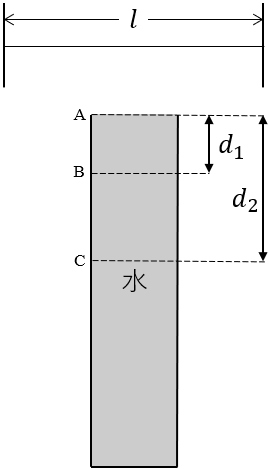
\includegraphics[width=\columnwidth]{../graphs/osaka_ko_23_3-1.png}
    \caption{}
  \end{minipage}
  \begin{minipage}{.25\columnwidth}
    \centering
    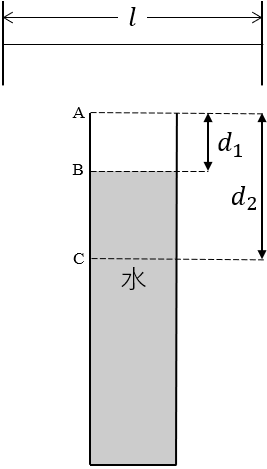
\includegraphics[width=\columnwidth]{../graphs/osaka_ko_23_3-2.png}
    \caption{}
  \end{minipage}
  \begin{minipage}{.25\columnwidth}
    \centering
    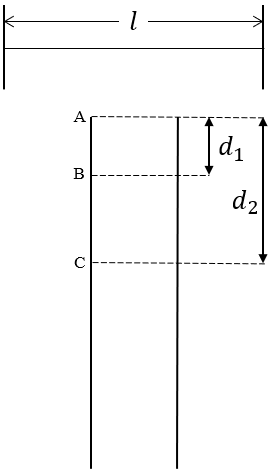
\includegraphics[width=\columnwidth]{../graphs/osaka_ko_23_3-3.png}
    \caption{}
  \end{minipage}
\end{figure}


% メモ
\begin{comment}

\end{comment}


%%%%%%%%%%%%%%%%%%
